\chapter{Smart Contract and Distributed Ledger Technology}
With the advances in technologies, transferring money is done over networks, and we just need to update related database entries that are controlled by central authorities like banks. These all processes need to third party to make appropriate transactions between unknown parties. \\
There are many problems with having third parties such as controlling the whole transaction by single authority, invalidating any transaction to serves their purpose . All these issues can be resolved using the novel idea of a distributed ledger. In this new technology, the third parties is eliminated, and all transactions will be done over the public network between parties within minutes. \\
With the presence of new technology, no one can manipulate transactions stored in a ledger or trace the involved parties in these transactions \cite {Masood}. 
\section{Ledger} 
A ledger is a book or computer that records transactions associated with a financial system. There are two different ledgers as below: \\
\textbf{Centralized Ledger} contains all recording transactions related to company assets, costs, libraries, etc. \\
\textbf{Decentralized Ledger} is a database that shares data across the network. It allows transactions to be executed in public. Any participant of each node can have an identical copy of the ledger, which is already shared on the network.\\
If any change or update occurs on the ledger, each node constructs a new transition and votes by the consensus algorithm to choose the correct copy of the ledger. Once the consensus has been done, other nodes will be synchronized with the latest version of the ledger \cite{Markos}.

\section{Distributed Vs. Decentralized } 
The difference between decentralized and distributed is made by Baran (1964) \cite{Baran}. Decentralized means that there is no single authority to make a decision. Each participant can make a decision individually, and the system gathers all responses as resulting behavior. However, there is no single authority in the distributed system too, but the process is spread across all participants and decisions will be centralized. The main difference between distributed and decentralized is that a decentralized database is a collection of inter-connected databases that work independently in different locations. Ozsu et al. \cite{Ozsu} define a distributed database as a "collection of multiple, logically interrelated databases distributed over a computer network and distributed database makes a transparent distribution to all users" \cite{Ozsu}. Based on this definition, blockchain technology covers both types, as it appears as a single system to its users and performs a task across a network. Thus, blockchain is a form of a distributed database system \cite{Markos}.


\section{Distributed Ledger Technology (DLT)} 
DLT refers to a database that provides identical copies of shared data among participants which would be updated using a complex consensus mechanism between participants. It is used to reduce the costs and increase transparently, traceability, and speed of the process.\\
This technology involves many challenges, and some of them have not been resolved so far. The most common challenges of DLT concern scalability, inseparability, and data privacy \cite{Jose}. \\
\\
\textbf{How does DLT work?}\\
\\
DLT is the result of combining main three technologies:\\
\hspace{1cm}\textit{-  P2P}: all participants (nodes) act simultaneously as client and server, consuming and contributing resources.\\
\hspace{1cm}\textit{- Cryptography} is used to authenticate the identity of the participant and the information between the two parties. Using encryption helps prevent third parties from accessing information. \\
\hspace{1cm}\textit{- Consensus algorithm} allows network participants to come into agreement to add a new node (block) to the ledger \cite{Jose}.\\
\section{Blockchain} According to what World Bank Group \cite{Natarajan} referred, blockchain is the most popular distributed ledger that stores and publishes data in packages called "blocks". Each block contains information such as nonce, timestamp, block hash, and a hash pointer to the previous block in its header. Therefore, all these blocks are connected in a digital chain \cite{Natarajan}. \\
Luke et al. \cite{Luke} refer to blockchain as a list of blocks that are linked to each other and secured cryptography. The participants on networks have an identical copy of these records stored locally on the computers of all participants. Blockchain starts processing, when the user request transaction whether is a transaction, contract, or other information. The transaction is broadcast on P2P network of nodes. Following that, the verification process takes place where all of the nodes in the P2P network verify the transactions via the hashes which are generated by some algorithm. Once verification is completed, transaction detail will be stored in a block. Finally, a new block is added to a chain in a way that is permanent and unchangeable \cite{Luke}. The initial block in the blockchain known as \textit{Genesis} block, the other nodes will be added to the chain after the process of consensus between nodes. The consensus mechanism allows the blockchain to grow without fear of manipulating the information of blocks. Since the blocks contain transactions, the consensus process takes place in a predefined time interval. This interval is the duration of when the initiation of the transaction took place and the addition of the transaction into a blockchain. This confirmation time is varied based on block size, transaction, and consensus algorithm. There are different methods for consensus mechanism listed: 
\begin{itemize}
    \item Proof of Work (PoW): 
    It is a mechanism that ensures consensus is done without any central control. By the usage of this mechanism miners compete to complete their transaction first into blockchain and get rewards (e.g: Bitcoin, Ether).\\
    Miners (actors who participate in cryptocurrency transactions) connect to blockchain and accomplish tasks validating transactions to add new blocks by solving a cryptographic puzzle and anybody who completes their task sooner can add their block first in blockchain \cite{Pablo}.
    \item Proof of Stake (PoS): 
    It is an alternative to proof-of-work that fewer CPU computations for mining. In proof of stake, the chance of mining the next block depends on node balance. 
    In private networks, however, where the participants know each other, consensus mechanisms such as proof of work are not required. This particularly removes the need for mining and gives us more variety of consensus protocols for picking from \cite{Christidis}.
    \item Proof of Authority (PoA): It confirms accounts and allows them to add a transaction in blocks. Since this approach is much more centralized and transaction speed is faster, is prone to be attacked more than the other methods \cite{Luke}.
    \item Practical Byzantine Fault Tolerance (PBFT): Blockchain tries to solve the problem called 'Byzantine Generals' which refers to some members on the network who send incoherent or fake information related to the transaction to others. Since there is no authority on blockchain to correct them, leads to the unreliability of blockchain. PBFT algorithm tries to achieve a consensus to solve this issue in a way that uses the concept of primary and secondary vote. Secondary vote automatically evaluate the decisions made by primary vote and can collectively change to a new primary, if primary vote is compromised \cite{Luke}.
\end{itemize}
Blockchain is associated with cryptocurrencies like Ethereum, bitcoin, lite coin, etc. Gupta (2017) \cite{Gupta} identified five core attributes which blockchain builds trust through them:
\begin{itemize}
    \item Distributed ledger: The data is not controlled by any single authority. It is shared, and updated across the network and the new changes will be replicated to all participants.
    \item Orchestrated and flexible: Since smart contracts can be executed on the blockchain. The blockchain can be evolved to support business processes and activities.
    \item Transparent and auditable: There is no need for a third party or another authority, as all participants have access to the same ledger, verify transactions, and identify the owner. 
    \item Secure, private, and indelible:
    Blockchain provides these features using some capabilities such as permissions and cryptography which ensures that  
    unauthorized users do not have any access to the network. It means that participants are really who they claim.
    \item Consensus: All nodes on the network should agree to validate transition and blockchain perform this process by consensus algorithm \cite{Gupta}.
\end{itemize}
\\
\textbf{Type of Blockchain} \\
\\
According to Aithal et al. \cite{Aithal} blockchain is used to transfer and exchange information through the secure network. Primarily, there were two types of blockchain technology: public and private networks. Based on some other analysis, blockchain can also be noted as consortium blockchain technology and hybrid blockchain technology \cite{Aithal}. \\
That should be noted that all kinds of blockchains consist of nodes and works on P2P peer-to-peer network. Aithal et al. \cite{Aithal} classified blockchain into three types as bellow: public blockchain, private blockchain, and consortium blockchain. Besides this, there is another type of blockchain, known as the hybrid blockchain.
\begin{itemize}
    \item \textbf{Public Blockchain} is the main type of blockchain that, is decentralized and open naturaly. In this system, anyone is allowed to join to network and create consensuses. In a public blockchain, any miner (participant) can create consensus mechanisms such as proof of work, and proof of stake to validate the transaction with a low rate of validity \cite{Kalra}.
    \item \textbf{Private Blockchain} is not open and restricted in a way that the only restricted participant has the right to validate the transaction. Therefore, it provides better privacy, improves scalability, and mitigates security issues. This blockchain does not have mining computation to reach the consensus because all participants are known in this network \cite{Kalra}. 
    \item \textbf{Consortium Blockchain} is semi-decentralized blockchain and is used to do activities for a single organization like bank, etc. The difference between private blockchain with this type is that Consortium Blockchain is controlled by a group rather than a single authority \cite{Aithal}.
    \item \textbf{Hybrid Blockchain} is a combination of public and private blockchains. Thus, it makes the benefit of privacy in private blockchain combined with the security and transparency of the public blockchain. In this type of blockchain, the user can control who gets access to which data on the blockchain. A transaction can be verified in a private network, and the user can release it to the public blockchain. By doing so, only selected parts of the records can be accessible in public and the rest could still maintain confidential in a private network \cite{Aithal}. 
\end{itemize}

 \section{Ethereum}
Ethereum is the most active public blockchain in the world at present. It is another cryptocurrency similar to Bitcoin that is built on top of the blockchain. The participant publishes the transactions on the network, which are then stored in blocks and added to the blockchain using a consensus mechanism. The term state in Ethereum refers to the state of different accounts pupulating on the blockchain. An account in Ethereum can either be an external account related to the user or a contract account that obtains constant storage in the blockchain. The virtual currency in this system is \textit{Ether}. The transaction can change the state of the system by creating a new contract or invoking an existing contract \cite{Ilya}.

\section{How does Ethereum works?}
In this subsection, we will focus on the Ethereum workflow at a technical level.
\subsection{Blockchain}
The blockchain contains some information that we have used in our project. Therefore we focus on it more, as below:
\begin{center}
	\begin{figure}[htb!]
		
		\begin{minipage}{0.5\linewidth}
			\centering
			\includegraphics[width=1.95\textwidth]{images/chap01_Blockchain.png}
		\end{minipage}
		\caption[Block contents]{Block contents \footnote{https://archive.researchworld.com/three-ways-that-blockchain-can-improve-the-quality-of-market-research/}}
		
	\end{figure}
	
\end{center}
\begin{itemize}
    \item \textbf{Block} as a data structure within the blockchain contains different functions which include transaction hashes and some other additional information for blockchain technology. Gavin Wood et al. \cite{Gavin} described some relevant information below and we used this information in our project: \\
    \begin{itemize}
        \item \textit{parentHash} is the hash of the parent block’s header.
        \item \textit{sateRoot} is the hash of the root node of the state, after execution of all transactions are applied.
        \item \textit{transactionRoot} is the hash of the root node of data populated with a transaction in the transactions list inside the block.
        \item \textit{receiptRoot}is the hash of the root node of the data populated with the receipts of transactions in the block.
        \item \textit{logsBloom} composed of log information.
        \item \textit{difficulty} represents the difficulty level of the block.
        \item \textit{number} is the number of ancestor blocks.
        \item \textit{gasLimit} represents the current limit of gas in the block.
        \item \textit{gasUsed} is the amount of gas used for the transaction in the block.
        \item \textit{timestamp} is time of reasonable output.
        \item \textit{extraData} is a byte array containing relevant information in the block.
        \item \textit{nonce} is number of several computations that have been done in the block.
    \end{itemize}
  \item \textbf{Mining} is a process of computation on the blockchain to verify and add a block. The miner adds a new block, and others check the validity of the new block. Any participant can take part in the mining pool, but the chance of finding a valid block depends on the power of the computer to perform calculations. Sometimes a miner will find an uncle block. 'An uncle block is a block that is initially valid but is surpassed by another faster block'. An Uncle block is rewarded with $\frac{7}{8}$ of full block value, and a hash will be added to a valid block. A maximum of two uncle blocks can be added to a valid block, and the miner of the valid block also receives $\frac{1}{32}$ extra Ether for each uncle block \cite{Egbertsen}.
    \item \textbf{Mining pool} is a way that miners gather together, start mining, solve blocks, and win rewards, and then the reward will be split among the involved miners \cite{Egbertsen}.
\end{itemize}
\subsection{Ether}
It is the form of payment and fuel for Ethereum. The base for mining (finding the solution and adding blocks) successfully is five ethers. If the miner finds a solution but not fast enough, it becomes less ether, like 4.375 ether, and will be an uncle block. Each block can contain just two uncle blocks and receive $\frac{1}{32}$ per uncle block. If another miner also finds a solution. This block cannot be added to the blockchain, and the miner just receives 2-3 ether \cite{Egbertsen}.
\subsection{Account}
There are two types of accounts in Ethereum:\\
- \textit{Normal account} is controlled by the private key. The owner of this account can send ether or a message.\\
- \textit{Contract} account is controlled by code. It can only fire a transaction in response to other transactions \cite{Egbertsen}. An account encompasses four fields:\\
 \begin{itemize}
     \item \textit{nonce} is the number of transactions sent from this address \cite{Gavin}.
     \item \textit{balance} is the number of Wei owned by this address \cite{Gavin}.
     \item \textit{storageRoot} is the hash of the root node of the Merkle Patrica tree, which encodes the content of an account. It should also be noted that the Merkle tree is used for data representation in the block header \cite{Gavin}.
     \item \textit{codeHash}
     is the hash associated with this account that would be executed when this account address receives a message call and would not be changeable anymore. All information about this account is stored in the database under the corresponding hash code for later retrieval \cite{Gavin}. \\
    
\end{itemize}
\textbf{Hash function}
is the process of SHA3 standardization at National Institute of Standards and Technology (NIST) was completed in August 2015.
This standard specifies the SHA3 (Secure Hash Algorithm-3) family of functions for binary data. Each hash function is based on \textit{Kacak} algorithm, known as NIST, the winner of the SHA3 cryptographic hash algorithm competition. The SHA3 family includes four functions with different lengths of 224, 256, 384, and 512 bits.
In the hash function, input is called as \textit{message} and output is called as \textit{has value} where the length of the message can vary but the length of the hash value is always fixed \cite{Dworkin}.\\


\begin{center}
	\begin{figure}[htb!]
		
		\begin{minipage}{0.2\linewidth}
			\centering
			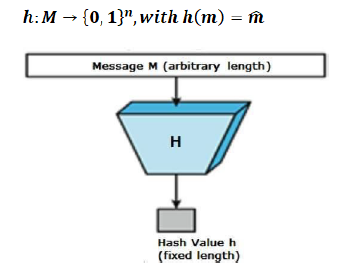
\includegraphics[width=4.5\textwidth]{images/chap01_hash_function.png}
		\end{minipage}
		\caption[Image of hash function]{Image of hash function \cite{Dworkin}}
		
	\end{figure}
	
\end{center}
\textbf{Gas} is fuel on the Ethereum platform that is paid before executing a transaction. In a case that the transaction is rolled back, the consumed gas will not be returned \cite{Egbertsen}.\\
\begin{itemize}
    \item \textbf{Transaction}
     Gavin Wood et al. \cite{Gavin} described a transaction as a cryptography-signed instruction that is executed by an external actor, which can be a human or another contract. The transaction describes these fields:
     \begin{itemize}
         \item \textit{nonce} is the number of transactions sent by the sender.
         \item \textit{gasPrice} is the number of wei to be paid per unit of gas.
         \item \textit{gasLimit} is the amount of gas that can be used for transactions.
         \item \textit{to} is the address to which that contract sends a transaction.
         \item \textit{value} is the number of wei that is transferred in the transaction.
     \end{itemize}
        \item \textbf{Message} is fired by contract and contains all attributes the same as a transaction, but $gasPrice$ \cite{Egbertsen}.
\end{itemize}
\subsection{Contract} 
It is an account on the Ethereum blockchain that has its own code and is controlled by code. The code inside the contract is triggered whenever it receives a message, allowing it to read and write contract storage or send a message. \\
A contract in Ethereum is an autonomous agent that performs some operations that are programmed to fulfill the user's goals, meaning that the contract is an autonomous agent that is executed when it receives a message or transaction, having control over its balance and the key/value store as constant variables.
The keys and values stored in the contract are long-lasting and get used whenever the contract starts running \cite{Egbertsen}.

\subsection{Smart Contract}
The term smart contract was coined in 1994 by Nick Szabo \cite{Szabo} who released that DLT can also be used for smart contracts.
According to Nick Szabo \textit{"Smart contract is a computerized transaction protocol that executes the terms of a contract"}\footnote{https://www.fon.hum.uva.nl/rob/Courses/InformationInSpeech/CDROM/Literature/LOTwinterschool2006/szabo.best.vwh.net/smart.contracts.html}. He visualized an away to write agreement that enforces the conditions between parties involved in a transaction automatically and more efficiently.
Smart contracts are run by each node as part of the block creation process. Block creation occurs when transactions take place in the block.
An important part of a smart contract is that each contract has its own address. Since the contract code is carried to the transaction, a node can create the specific transaction, assigning an address to the contract, and this transaction is capable of running contract code at the time of creation.\\
After that, the contract will be part of the block, and the address will never change. Whenever the node wants to call a method inside the contract, it should send a message to the address of the contract that has the method and input data.
The contract will run as part of the creation of a new block and then return value or store data on the blockchain \cite{Payrott}.\\
\\
\textbf{Solidity} is a high-level, truing complete language with a Java script similar syntax. The contract is similar to classes in an object-oriented language, which contain fields for persistent storage of contracts and methods to be invoked by internal and external transactions. For interacting with another contract, we either need to create a new instance of this contract or make a transaction to a known contract address.\\
In principle, Solidity provides some basics to access blocks and transaction details, like: \textit{msg:sender} for accessing the address of an account or \textit{msg:value} to access the amount of \textit{wei} transferred by the transaction. It also uses some functions to transfer money to another contract, such as \textit{call} and \textit{send}. These functions get used to transfer value and translate into an internal call to a transaction, which causes the contract to also execute code or may fail to execute due to insufficient gas \cite{Ilya}.